% Options for packages loaded elsewhere
\PassOptionsToPackage{unicode}{hyperref}
\PassOptionsToPackage{hyphens}{url}
%
\documentclass[
  14pt,
  ignorenonframetext,
]{beamer}
\usepackage{pgfpages}
\setbeamertemplate{caption}[numbered]
\setbeamertemplate{caption label separator}{: }
\setbeamercolor{caption name}{fg=normal text.fg}
\beamertemplatenavigationsymbolsempty
% Prevent slide breaks in the middle of a paragraph
\widowpenalties 1 10000
\raggedbottom
\setbeamertemplate{part page}{
  \centering
  \begin{beamercolorbox}[sep=16pt,center]{part title}
    \usebeamerfont{part title}\insertpart\par
  \end{beamercolorbox}
}
\setbeamertemplate{section page}{
  \centering
  \begin{beamercolorbox}[sep=12pt,center]{part title}
    \usebeamerfont{section title}\insertsection\par
  \end{beamercolorbox}
}
\setbeamertemplate{subsection page}{
  \centering
  \begin{beamercolorbox}[sep=8pt,center]{part title}
    \usebeamerfont{subsection title}\insertsubsection\par
  \end{beamercolorbox}
}
\AtBeginPart{
  \frame{\partpage}
}
\AtBeginSection{
  \ifbibliography
  \else
    \frame{\sectionpage}
  \fi
}
\AtBeginSubsection{
  \frame{\subsectionpage}
}
\usepackage{lmodern}
\usepackage{amssymb,amsmath}
\usepackage{ifxetex,ifluatex}
\ifnum 0\ifxetex 1\fi\ifluatex 1\fi=0 % if pdftex
  \usepackage[T1]{fontenc}
  \usepackage[utf8]{inputenc}
  \usepackage{textcomp} % provide euro and other symbols
\else % if luatex or xetex
  \usepackage{unicode-math}
  \defaultfontfeatures{Scale=MatchLowercase}
  \defaultfontfeatures[\rmfamily]{Ligatures=TeX,Scale=1}
\fi
% Use upquote if available, for straight quotes in verbatim environments
\IfFileExists{upquote.sty}{\usepackage{upquote}}{}
\IfFileExists{microtype.sty}{% use microtype if available
  \usepackage[]{microtype}
  \UseMicrotypeSet[protrusion]{basicmath} % disable protrusion for tt fonts
}{}
\makeatletter
\@ifundefined{KOMAClassName}{% if non-KOMA class
  \IfFileExists{parskip.sty}{%
    \usepackage{parskip}
  }{% else
    \setlength{\parindent}{0pt}
    \setlength{\parskip}{6pt plus 2pt minus 1pt}}
}{% if KOMA class
  \KOMAoptions{parskip=half}}
\makeatother
\usepackage{xcolor}
\IfFileExists{xurl.sty}{\usepackage{xurl}}{} % add URL line breaks if available
\IfFileExists{bookmark.sty}{\usepackage{bookmark}}{\usepackage{hyperref}}
\hypersetup{
  pdftitle={R Markdownで日本語プレゼンテーション},
  pdfauthor={ill-identified},
  hidelinks,
  pdfcreator={LaTeX via pandoc}}
\urlstyle{same} % disable monospaced font for URLs
\newif\ifbibliography
\usepackage{color}
\usepackage{fancyvrb}
\newcommand{\VerbBar}{|}
\newcommand{\VERB}{\Verb[commandchars=\\\{\}]}
\DefineVerbatimEnvironment{Highlighting}{Verbatim}{commandchars=\\\{\}}
% Add ',fontsize=\small' for more characters per line
\usepackage{framed}
\definecolor{shadecolor}{RGB}{248,248,248}
\newenvironment{Shaded}{\begin{snugshade}}{\end{snugshade}}
\newcommand{\AlertTok}[1]{\textcolor[rgb]{0.94,0.16,0.16}{#1}}
\newcommand{\AnnotationTok}[1]{\textcolor[rgb]{0.56,0.35,0.01}{\textbf{\textit{#1}}}}
\newcommand{\AttributeTok}[1]{\textcolor[rgb]{0.77,0.63,0.00}{#1}}
\newcommand{\BaseNTok}[1]{\textcolor[rgb]{0.00,0.00,0.81}{#1}}
\newcommand{\BuiltInTok}[1]{#1}
\newcommand{\CharTok}[1]{\textcolor[rgb]{0.31,0.60,0.02}{#1}}
\newcommand{\CommentTok}[1]{\textcolor[rgb]{0.56,0.35,0.01}{\textit{#1}}}
\newcommand{\CommentVarTok}[1]{\textcolor[rgb]{0.56,0.35,0.01}{\textbf{\textit{#1}}}}
\newcommand{\ConstantTok}[1]{\textcolor[rgb]{0.00,0.00,0.00}{#1}}
\newcommand{\ControlFlowTok}[1]{\textcolor[rgb]{0.13,0.29,0.53}{\textbf{#1}}}
\newcommand{\DataTypeTok}[1]{\textcolor[rgb]{0.13,0.29,0.53}{#1}}
\newcommand{\DecValTok}[1]{\textcolor[rgb]{0.00,0.00,0.81}{#1}}
\newcommand{\DocumentationTok}[1]{\textcolor[rgb]{0.56,0.35,0.01}{\textbf{\textit{#1}}}}
\newcommand{\ErrorTok}[1]{\textcolor[rgb]{0.64,0.00,0.00}{\textbf{#1}}}
\newcommand{\ExtensionTok}[1]{#1}
\newcommand{\FloatTok}[1]{\textcolor[rgb]{0.00,0.00,0.81}{#1}}
\newcommand{\FunctionTok}[1]{\textcolor[rgb]{0.00,0.00,0.00}{#1}}
\newcommand{\ImportTok}[1]{#1}
\newcommand{\InformationTok}[1]{\textcolor[rgb]{0.56,0.35,0.01}{\textbf{\textit{#1}}}}
\newcommand{\KeywordTok}[1]{\textcolor[rgb]{0.13,0.29,0.53}{\textbf{#1}}}
\newcommand{\NormalTok}[1]{#1}
\newcommand{\OperatorTok}[1]{\textcolor[rgb]{0.81,0.36,0.00}{\textbf{#1}}}
\newcommand{\OtherTok}[1]{\textcolor[rgb]{0.56,0.35,0.01}{#1}}
\newcommand{\PreprocessorTok}[1]{\textcolor[rgb]{0.56,0.35,0.01}{\textit{#1}}}
\newcommand{\RegionMarkerTok}[1]{#1}
\newcommand{\SpecialCharTok}[1]{\textcolor[rgb]{0.00,0.00,0.00}{#1}}
\newcommand{\SpecialStringTok}[1]{\textcolor[rgb]{0.31,0.60,0.02}{#1}}
\newcommand{\StringTok}[1]{\textcolor[rgb]{0.31,0.60,0.02}{#1}}
\newcommand{\VariableTok}[1]{\textcolor[rgb]{0.00,0.00,0.00}{#1}}
\newcommand{\VerbatimStringTok}[1]{\textcolor[rgb]{0.31,0.60,0.02}{#1}}
\newcommand{\WarningTok}[1]{\textcolor[rgb]{0.56,0.35,0.01}{\textbf{\textit{#1}}}}
\usepackage{longtable,booktabs}
\usepackage{caption}
% Make caption package work with longtable
\makeatletter
\def\fnum@table{\tablename~\thetable}
\makeatother
\usepackage{graphicx,grffile}
\makeatletter
\def\maxwidth{\ifdim\Gin@nat@width>\linewidth\linewidth\else\Gin@nat@width\fi}
\def\maxheight{\ifdim\Gin@nat@height>\textheight\textheight\else\Gin@nat@height\fi}
\makeatother
% Scale images if necessary, so that they will not overflow the page
% margins by default, and it is still possible to overwrite the defaults
% using explicit options in \includegraphics[width, height, ...]{}
\setkeys{Gin}{width=\maxwidth,height=\maxheight,keepaspectratio}
% Set default figure placement to htbp
\makeatletter
\def\fps@figure{htbp}
\makeatother
\usepackage[normalem]{ulem}
% Avoid problems with \sout in headers with hyperref
\pdfstringdefDisableCommands{\renewcommand{\sout}{}}
\setlength{\emergencystretch}{3em} % prevent overfull lines
\providecommand{\tightlist}{%
  \setlength{\itemsep}{0pt}\setlength{\parskip}{0pt}}
\setcounter{secnumdepth}{-\maxdimen} % remove section numbering
\usetheme[progressbar=frametitle,block=fill]{metropolis}
\makeatletter
\setlength{\metropolis@progressinheadfoot@linewidth}{2pt}
\usecolortheme{default}
\useoutertheme{default}
\useinnertheme{default}
\usefonttheme{professionalfonts}
\usepackage{zxjatype}
\setmainfont{Palatino Linotype}
\setsansfont{Arial}
\setmonofont{Ricty Diminished}
\setjamainfont{Noto Serif CJK JP}
\setjasansfont{Noto Sans CJK JP}
\setjamonofont{Ricty Diminished}
\usepackage {hyperref}
\hypersetup {colorlinks=true,linkcolor=blue,citecolor=blue,urlcolor=magenta}
\renewcommand{\figurename}{図}
\renewcommand{\tablename}{表}
\usepackage{bxtexlogo}
\colorlet{shadecolor}{gray!20}
\usepackage[numbers]{natbib}
\renewcommand{\bibsection}{}
\renewcommand*{\bibfont}{\footnotesize}
\usepackage{fmtcount}
\renewcommand{\theFancyVerbLine}{\small \padzeroes[2]{\decimal{FancyVerbLine}}}
\IfFileExists{bxcoloremoji.sty}{\usepackage{bxcoloremoji}}{}
\usepackage[]{natbib}
\bibliographystyle{jecon}

\title{R Markdownで日本語\texttt{beamer}プレゼンテーション}
\author{ill-identified}
\date{2020-06-21}

\begin{document}
\frame{\titlepage}

\begin{frame}
  \tableofcontents[hideallsubsections]
\end{frame}
\begin{frame}{要件}
\protect\hypertarget{ux8981ux4ef6}{}

\begin{itemize}
\tightlist
\item
  想定される用途

  \begin{itemize}
  \tightlist
  \item
    Tokyo.R などRを使った話を発表する際の資料作成
  \item
    技術・アカデミック寄りの話題を想定
  \end{itemize}
\item
  要求されるもの

  \begin{itemize}
  \tightlist
  \item
    \textbf{日本語表示}
  \item
    ラスタまたはベクタ画像の挿入
  \item
    表の挿入
  \item
    Rコードを見やすく表示
  \item
    参考文献の相互参照/リスト自動生成
  \item
    \textbf{LyX やoverleafより簡単であること}
  \item
    \textbf{なんかナウでオサレな感じは求めてない}

    \begin{itemize}
    \tightlist
    \item
      自由すぎるデザインは不可
    \end{itemize}
  \end{itemize}
\end{itemize}

\end{frame}

\begin{frame}{先行研究の紹介}
\protect\hypertarget{ux5148ux884cux7814ux7a76ux306eux7d39ux4ecb}{}

\begin{itemize}
\tightlist
\item
  伊東『\href{https://www.slideshare.net/hirokito/r-markdownbeamer-88777082}{R
  MarkdownとBeamerでプレゼンテーション資料作成}』

  \begin{itemize}
  \tightlist
  \item
    \LuaLaTeX を使って日本語でBeamerスライド作成する方法
  \end{itemize}
\item
  伊東先生の資料との違い:

  \begin{itemize}
  \tightlist
  \item
    エンジンを\XeLaTeX に変更
  \item
    日本語文献bibファイル・bstファイルに対応
  \item
    スライド作例を多少充実させた
  \item
    その他体裁にこだわりたい人向け

    \begin{itemize}
    \tightlist
    \item
      「表X」「図X」といったキャプション
    \end{itemize}
  \end{itemize}
\end{itemize}

\end{frame}

\begin{frame}{\texttt{reveal.js} じゃダメなの?}
\protect\hypertarget{reveal.js-ux3058ux3083ux30c0ux30e1ux306aux306e}{}

\begin{itemize}
\tightlist
\item
  個人的にデザインとかあまり好きじゃない
\item
  上下左右に動いて空間識失調になる

  \begin{itemize}
  \tightlist
  \item
    (個人の体験です)
  \item
    上下のみにもできる
  \end{itemize}
\item
  htmlよりも不変な媒体にしたい

  \begin{itemize}
  \tightlist
  \item
    pdfが明確に優れているかは怪しい
  \end{itemize}
\item
  \sout{Q: お前が使いこなせてないだけじゃないの?}

  \begin{itemize}
  \tightlist
  \item
    \sout{A: うるさい}
  \end{itemize}
\end{itemize}

\end{frame}

\begin{frame}[fragile]{パワーポイントじゃダメなの?}
\protect\hypertarget{ux30d1ux30efux30fcux30ddux30a4ux30f3ux30c8ux3058ux3083ux30c0ux30e1ux306aux306e}{}

\begin{itemize}
\tightlist
\item
  私は\textbf{持ってない}
\item
  シンタックスハイライトが面倒

  \begin{itemize}
  \tightlist
  \item
    パワポの場合は\href{https://notchained.hatenablog.com/entry/2017/02/20/221446}{VSCode}か\href{https://reprex.tidyverse.org/articles/articles/rtf.html}{\texttt{reprex}}でコピペ
  \end{itemize}
\item
  ドラッグ\&ドロップで位置調整は便利
\item
  しかしポンチ絵芸術になりがち
\item
  極力シンプルにして視線誘導の負担をなくすべき

  \begin{itemize}
  \tightlist
  \item
    徹底するかは好みの問題
  \end{itemize}
\end{itemize}

\end{frame}

\begin{frame}[fragile]{技術的に厄介だったところ}
\protect\hypertarget{ux6280ux8853ux7684ux306bux5384ux4ecbux3060ux3063ux305fux3068ux3053ux308d}{}

\begin{itemize}
\tightlist
\item
  htmlとpdf(\LaTeX)とで微妙に違う挙動

  \begin{itemize}
  \tightlist
  \item
    ネット上の情報はhtml前提が多い
  \item
    pandocチョットワカル必要
  \end{itemize}
\item
  日本語を含む参考文献リスト

  \begin{itemize}
  \tightlist
  \item
    \upBibTeX の適用
  \item
    細かいオプション, 特に\texttt{metropolis}特有の仕様
  \end{itemize}
\item
  RStudio Cloud で動くかは未確認

  \begin{itemize}
  \tightlist
  \item
    日本語表示がおかしい説あり
  \end{itemize}
\end{itemize}

\end{frame}

\hypertarget{ux4f7fux3044ux65b9}{%
\section{使い方}\label{ux4f7fux3044ux65b9}}

\begin{frame}{基本}
\protect\hypertarget{ux57faux672c}{}

\begin{enumerate}
\tightlist
\item
  RStudioのツールバーの``knit''
\item
  またはドロップダウンして``Knit to PDF (Beamer)''
\end{enumerate}

\begin{center}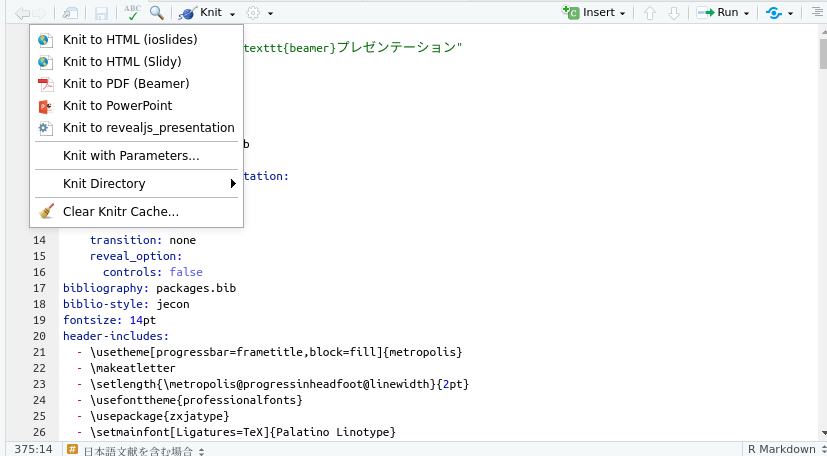
\includegraphics[width=0.9\linewidth]{img/render} \end{center}

\end{frame}

\begin{frame}[fragile]{フォント指定}
\protect\hypertarget{ux30d5ux30a9ux30f3ux30c8ux6307ux5b9a}{}

\begin{itemize}
\tightlist
\item
  以下の箇所を適当に変える
\item
  \texttt{set*font}は欧文用
\item
  \texttt{setja*font}は和文用
\item
  インラインでのフォント変更は\textbf{想定してない}

  \begin{itemize}
  \tightlist
  \item
    不可能ではないが面倒
  \end{itemize}
\end{itemize}

\begin{Shaded}
\begin{Highlighting}[]
\KeywordTok{-}\AttributeTok{ \textbackslash{}setmainfont\{Palatino Linotype\}}
\KeywordTok{-}\AttributeTok{ \textbackslash{}setsansfont\{Arial\}}
\KeywordTok{-}\AttributeTok{ \textbackslash{}setmonofont\{Ricty Diminished\}}
\KeywordTok{-}\AttributeTok{ \textbackslash{}setjamainfont\{Noto Serif CJK JP\}}
\KeywordTok{-}\AttributeTok{ \textbackslash{}setjasansfont\{Noto Sans CJK JP\}}
\KeywordTok{-}\AttributeTok{ \textbackslash{}setjamonofont\{Ricty Diminished\}}
\end{Highlighting}
\end{Shaded}

\end{frame}

\begin{frame}[fragile]{基本構文}
\protect\hypertarget{ux57faux672cux69cbux6587}{}

\begin{itemize}
\tightlist
\item
  markdown的な書き方でできる
\item
  ``\texttt{\#\#}タイトル'' でスライドの開始

  \begin{itemize}
  \tightlist
  \item
    \LaTeX コマンドも挿入可能
  \end{itemize}
\end{itemize}

\begin{Shaded}
\begin{Highlighting}[]
\FunctionTok{# 節見出し}
\FunctionTok{## タイトル1}
\NormalTok{- **太字**}
\NormalTok{- }\StringTok{_斜体_}
\StringTok{- }\BaseNTok{`タイプライタ体`}
\end{Highlighting}
\end{Shaded}

\begin{itemize}
\tightlist
\item
  \textbf{太字}
\item
  \emph{斜体}
\item
  \texttt{タイプライタ体}
\end{itemize}

\end{frame}

\begin{frame}{BeamerやRMarkdown使用に役立つ資料}
\protect\hypertarget{beamerux3084rmarkdownux4f7fux7528ux306bux5f79ux7acbux3064ux8cc7ux6599}{}

\begin{itemize}
\tightlist
\item
  伊東『\href{https://www.slideshare.net/hirokito/r-markdownbeamer-88777082}{R
  MarkdownとBeamerでプレゼンテーション資料作成}』(\LuaLaTeX 使用)
\item
  松田『\href{http://ayapin-film.sakura.ne.jp/LaTeX/slides.html\#beamer}{Beamer読本-講演用スライド作成のために-}』
\item
  Kazutan『\href{https://kazutan.github.io/SappoRoR6/rmd_slide.html\#/}{R
  Markdownによるスライド生成}』『\href{https://kazutan.github.io/kazutanR/Rmd_intro.html}{R
  Markdown入門}』
\item
  Atusy『\href{https://blog.atusy.net/2019/05/14/rmd2pdf-any-font/}{R
  Markdown + XeLaTeX で日本語含め好きなフォントを使って PDF
  を出力する}』
\item
  R Markdown 2.0
  チートシートの\href{https://rstudio.com/wp-content/uploads/2016/11/Rmarkdown-cheatsheet-2.0_ja.pdf}{日本語訳},
  Takahashi, M.訳
\end{itemize}

\end{frame}

\begin{frame}{もう少しくわしいやつ}
\protect\hypertarget{ux3082ux3046ux5c11ux3057ux304fux308fux3057ux3044ux3084ux3064}{}

\begin{itemize}
\tightlist
\item
  Atusy 『\href{https://atusy.booth.pm/items/1453002}{R
  MarkdownユーザーのためのPandoc's Markdown}』
\item
  謝益輝 (yihui) ``\href{https://yihui.org/knitr/}{knitr - Elegant,
  flexible, and fast dynamic report generation with R}'' (開発者本人)
\item
  Xie, Yihui \& C. Dervieux
  ``\href{https://bookdown.org/yihui/rmarkdown-cookbook/}{R Markdown
  Coobook}''
\end{itemize}

\begin{figure}

{\centering 
\includegraphics[width=0.5\linewidth,height=0.1\textheight]{img/yihui} 

}

\caption{謝益輝近影}\label{fig:yihui-logo}
\end{figure}

\end{frame}

\begin{frame}[fragile]{今回使うパッケージ}
\protect\hypertarget{ux4ecaux56deux4f7fux3046ux30d1ux30c3ux30b1ux30fcux30b8}{}

\begin{itemize}
\tightlist
\item
  このファイル作成には以下を使用している

  \begin{itemize}
  \tightlist
  \item
    図表作成とか最低限必要なものだけ
  \end{itemize}
\end{itemize}

\begin{Shaded}
\begin{Highlighting}[numbers=left,,]
\KeywordTok{require}\NormalTok{(conflicted)}
\KeywordTok{require}\NormalTok{(tidyverse)}
\KeywordTok{require}\NormalTok{(ggthemes)}
\KeywordTok{require}\NormalTok{(ggdag)}
\end{Highlighting}
\end{Shaded}

\begin{itemize}
\tightlist
\item
  以下はインストールのみ/読み込む必要なし

  \begin{itemize}
  \tightlist
  \item
    \texttt{citr}: 引用文献の挿入をGUIで
  \item
    \texttt{bookdown}: 数式をGUIで
  \end{itemize}
\end{itemize}

\end{frame}

\begin{frame}[fragile]{ソースコードの表示: 基本事項}
\protect\hypertarget{ux30bdux30fcux30b9ux30b3ux30fcux30c9ux306eux8868ux793a-ux57faux672cux4e8bux9805}{}

\begin{itemize}
\tightlist
\item
  \texttt{echo=T}でチャンク内コードを表示

  \begin{itemize}
  \tightlist
  \item
    デフォでは非表示
  \item
    \textbf{自動でシンタックスハイライト}
  \end{itemize}
\item
  はみ出す場合は\texttt{tidy=F}して手動改行

  \begin{itemize}
  \tightlist
  \item
    日本語等で折り返し地点がうまく行かない
  \end{itemize}
\item
  \texttt{class.source\ =\ "numberLines,\ LineAnchors"}
  で行番号表示(\href{https://blog.atusy.net/2019/04/18/rmd-line-num/}{参考})
\end{itemize}

\end{frame}

\begin{frame}[fragile]{ソースコードの表示: 出力例}
\protect\hypertarget{ux30bdux30fcux30b9ux30b3ux30fcux30c9ux306eux8868ux793a-ux51faux529bux4f8b}{}

\begin{verbatim}
```{r, echo=T, class.source = "numberLines, LineAnchors"}
require(conflicted)
require(tidyverse)
require(ggthemes)
require(ggdag)
```
\end{verbatim}

\begin{Shaded}
\begin{Highlighting}[numbers=left,,]
\KeywordTok{require}\NormalTok{(conflicted)}
\KeywordTok{require}\NormalTok{(tidyverse)}
\KeywordTok{require}\NormalTok{(ggthemes)}
\KeywordTok{require}\NormalTok{(ggdag)}
\end{Highlighting}
\end{Shaded}

\end{frame}

\hypertarget{ux6570ux5f0fux95a2ux4fc2}{%
\section{数式関係}\label{ux6570ux5f0fux95a2ux4fc2}}

\begin{frame}[fragile]{数式の挿入: 行内(インライン)}
\protect\hypertarget{ux6570ux5f0fux306eux633fux5165-ux884cux5185ux30a4ux30f3ux30e9ux30a4ux30f3}{}

\begin{itemize}
\tightlist
\item
  markdown風のLaTeXコード埋め込み
\item
  \LaTeX の数式を\texttt{\$}で挟む
\item
  例: \texttt{らんま\$\textbackslash{}frac\{1\}\{2\}\$}

  \begin{itemize}
  \tightlist
  \item
    出力: らんま\(\frac{1}{2}\)
  \item
    注: 行内で分数はスラッシュ使ったほうが見やすい
  \end{itemize}
\item
  セリフフォント使用

  \begin{itemize}
  \tightlist
  \item
    スライドはサンセリフが良いとされる
  \item
    しかし数式の統一感がない
  \item
    (個人の好み?)
  \end{itemize}
\end{itemize}

\end{frame}

\begin{frame}[fragile]{数式の挿入: 独立行}
\protect\hypertarget{ux6570ux5f0fux306eux633fux5165-ux72ecux7acbux884c}{}

\begin{itemize}
\tightlist
\item
  \texttt{\$\$}で挟んだ範囲に\LaTeX 構文
\end{itemize}

\begin{Shaded}
\begin{Highlighting}[]
\SpecialStringTok{$$}\SpecialCharTok{\textbackslash{}begin}\SpecialStringTok{\{aligned\}}
\SpecialStringTok{& }\SpecialCharTok{\textbackslash{}sin}\SpecialStringTok{^2(x) + }\SpecialCharTok{\textbackslash{}cos}\SpecialStringTok{^2(x) = 1}\SpecialCharTok{\textbackslash{}\textbackslash{}}
\SpecialStringTok{& f(x) = }\SpecialCharTok{\textbackslash{}frac}\SpecialStringTok{\{1\}\{(2}\SpecialCharTok{\textbackslash{}pi}\SpecialStringTok{)^2\}}\SpecialCharTok{\textbackslash{}int}\SpecialStringTok{_\{}\SpecialCharTok{\textbackslash{}mathbb}\SpecialStringTok{\{R\}^n\}}
\SpecialCharTok{\textbackslash{}hat}\SpecialStringTok{\{f\}(}\SpecialCharTok{\textbackslash{}omega}\SpecialStringTok{)}\SpecialCharTok{\textbackslash{}exp}\SpecialStringTok{(i}\SpecialCharTok{\textbackslash{}omega}\SpecialStringTok{ x)d}\SpecialCharTok{\textbackslash{}omega}
\SpecialCharTok{\textbackslash{}end}\SpecialStringTok{\{aligned\}$$}
\end{Highlighting}
\end{Shaded}

\[\begin{aligned}
& \sin^2(x) + \cos^2(x) = 1\\
& f(x) = \frac{1}{(2\pi)^2}\int_{\mathbb{R}^n}\hat{f}(\omega)\exp(i\omega x)d\omega
\end{aligned}\]

\end{frame}

\begin{frame}[fragile]{数式の挿入: \texttt{bookdown} の使用}
\protect\hypertarget{ux6570ux5f0fux306eux633fux5165-bookdown-ux306eux4f7fux7528}{}

\begin{enumerate}
\tightlist
\item
  RStudioのツールバー ``Addins''
\item
  ``Input LaTeX Math''
\end{enumerate}

\begin{figure}

{\centering 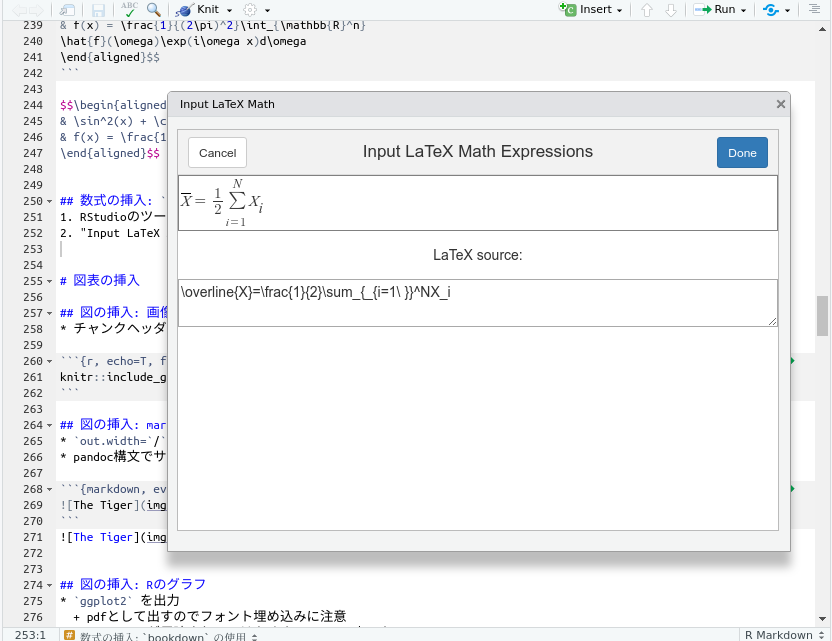
\includegraphics[width=0.5\linewidth,height=0.4\textheight]{img/math-input} 

}

\caption{bookdownの数式入力機能}\label{fig:math-input}
\end{figure}

\begin{itemize}
\tightlist
\item
  一部対応してない記号もある?

  \begin{itemize}
  \tightlist
  \item
    \texttt{\textbackslash{}mathbb\{\}}とか\texttt{\textbackslash{}hat\{\}}とか
  \end{itemize}
\item
  数式のみで\texttt{\textbackslash{}aligned}等環境の入力は不可
\end{itemize}

\end{frame}

\hypertarget{ux56f3ux8868ux306eux633fux5165}{%
\section{図表の挿入}\label{ux56f3ux8868ux306eux633fux5165}}

\begin{frame}[fragile]{図の挿入: 画像ファイル貼り付け}
\protect\hypertarget{ux56f3ux306eux633fux5165-ux753bux50cfux30d5ux30a1ux30a4ux30ebux8cbcux308aux4ed8ux3051}{}

\begin{itemize}
\tightlist
\item
  チャンクヘッダの\texttt{out.width=}/\texttt{out.height=}でサイズ調整
\end{itemize}

\begin{Shaded}
\begin{Highlighting}[]
\NormalTok{knitr}\OperatorTok{::}\KeywordTok{include_graphics}\NormalTok{(}\KeywordTok{c}\NormalTok{(}\StringTok{"img/tiger.eps"}\NormalTok{, }
    \StringTok{"img/tiger.pdf"}\NormalTok{, }\StringTok{"img/tiger.png"}\NormalTok{))}
\end{Highlighting}
\end{Shaded}

\begin{figure}

{\centering 
\includegraphics[width=0.2\linewidth]{img/tiger} 
\includegraphics[width=0.2\linewidth]{img/tiger} 
\includegraphics[width=0.2\linewidth]{img/tiger} 

}

\caption{いつもの虎(TeXLiveより)}\label{fig:unnamed-chunk-3}
\end{figure}

\end{frame}

\begin{frame}[fragile]{図の挿入: markdown構文で貼り付け}
\protect\hypertarget{ux56f3ux306eux633fux5165-markdownux69cbux6587ux3067ux8cbcux308aux4ed8ux3051}{}

\begin{itemize}
\tightlist
\item
  \texttt{out.width=}/\texttt{out.height=}が適用されない
\item
  pandoc構文でサイズ指定
\end{itemize}

\begin{Shaded}
\begin{Highlighting}[]
\AlertTok{![The Tiger](img/tiger.pdf)}\NormalTok{\{ height=30% \}}
\end{Highlighting}
\end{Shaded}

\begin{figure}
\centering

\includegraphics[width=\textwidth,height=0.3\textheight]{img/tiger.pdf}
\caption{The Tiger}
\end{figure}

\end{frame}

\begin{frame}[fragile]{図の挿入: Rのグラフ}
\protect\hypertarget{ux56f3ux306eux633fux5165-rux306eux30b0ux30e9ux30d5}{}

\begin{itemize}
\tightlist
\item
  \texttt{ggplot2} を出力

  \begin{itemize}
  \tightlist
  \item
    pdfとして出すのでフォント埋め込みに注意
  \item
    \texttt{theme()}が反映されるのはあくまでRStudio上のもの
  \item
    pdfでは相対的フォントサイズが変わる問題
  \end{itemize}
\end{itemize}

\begin{figure}

{\centering \includegraphics[width=0.5\linewidth]{presen_test_files/figure-beamer/plot-example-1} 

}

\caption{ggplot2の出力例: irisデータ}\label{fig:plot-example}
\end{figure}

\end{frame}

\begin{frame}[fragile]{図の挿入: 再現可能なポンチ絵}
\protect\hypertarget{ux56f3ux306eux633fux5165-ux518dux73feux53efux80fdux306aux30ddux30f3ux30c1ux7d75}{}

\begin{itemize}
\tightlist
\item
  概念図とかの図示はどうするか

  \begin{itemize}
  \tightlist
  \item
    NOT データの視覚化(ビジュアライゼーション)
  \item
    \texttt{ggplot2}の本来の使い方ではない
  \end{itemize}
\item
  \texttt{ggdag} はネットワーク図に使える

  \begin{itemize}
  \tightlist
  \item
    因果ダイアグラム, 遷移図, グラフィカルモデル等
  \end{itemize}
\item
  \texttt{ggforce}
  は\href{https://rpubs.com/sdutky/559050}{ベン図の描画に応用可能}

  \begin{itemize}
  \tightlist
  \item
    世間的にはグラフの部分拡大用パッケージ?
  \end{itemize}
\item
  詳しくは個別のマニュアル参照
\item
  霞が関流ポンチ絵は\textbf{専門外}
\end{itemize}

\end{frame}

\begin{frame}{図の挿入: ポンチ絵の例1}
\protect\hypertarget{ux56f3ux306eux633fux5165-ux30ddux30f3ux30c1ux7d75ux306eux4f8b1}{}

\begin{itemize}
\tightlist
\item
  \href{https://speakerdeck.com/ktgrstsh/r-and-epidemical-mathematical-models}{以前作ったやつ}の転載
\end{itemize}

\begin{figure}

{\centering \includegraphics[width=0.9\linewidth,height=0.7\textheight]{presen_test_files/figure-beamer/punch-chart-example-1} 

}

\caption{ggdagで作ったYJ-SEIRモデルの遷移図}\label{fig:punch-chart-example}
\end{figure}

\end{frame}

\begin{frame}[fragile]{図の挿入: ポンチ絵の例2}
\protect\hypertarget{ux56f3ux306eux633fux5165-ux30ddux30f3ux30c1ux7d75ux306eux4f8b2}{}

\begin{itemize}
\tightlist
\item
  \texttt{ggforce::geom\_circle()} を利用

  \begin{itemize}
  \tightlist
  \item
    参考:
    \href{https://scriptsandstatistics.wordpress.com/2018/04/26/how-to-plot-venn-diagrams-using-r-ggplot2-and-ggforce/}{How
    to Plot Venn Diagrams Using R, ggplot2 and ggforce}
  \end{itemize}
\end{itemize}

\begin{figure}

{\centering \includegraphics[width=0.5\linewidth]{presen_test_files/figure-beamer/venn-1} 

}

\caption{ベン図の例}\label{fig:venn}
\end{figure}

\end{frame}

\begin{frame}[fragile]{表の挿入: データフレーム}
\protect\hypertarget{ux8868ux306eux633fux5165-ux30c7ux30fcux30bfux30d5ux30ecux30fcux30e0}{}

\begin{itemize}
\tightlist
\item
  Rのデータフレームとして作成して出す

  \begin{itemize}
  \tightlist
  \item
    はみ出す場合は縮小
  \item
    最低限の情報だけ掲載するのは大前提
  \item
    \texttt{df\_print:\ kable}
    では\texttt{caption}指定が\href{https://stackoverflow.com/questions/48410861/how-to-add-table-caption-using-df-print}{ややこしい}
  \end{itemize}
\end{itemize}

\begin{Shaded}
\begin{Highlighting}[]
\KeywordTok{data}\NormalTok{(iris)}
\NormalTok{knitr}\OperatorTok{::}\KeywordTok{kable}\NormalTok{(}\KeywordTok{head}\NormalTok{(iris[, }\DecValTok{1}\OperatorTok{:}\DecValTok{3}\NormalTok{]),}
             \DataTypeTok{caption=}\StringTok{"kable()による表示"}\NormalTok{)}
\end{Highlighting}
\end{Shaded}

\end{frame}

\begin{frame}[fragile]{表の挿入: データフレームを\texttt{kable()}で表示}
\protect\hypertarget{ux8868ux306eux633fux5165-ux30c7ux30fcux30bfux30d5ux30ecux30fcux30e0ux3092kableux3067ux8868ux793a}{}

\begin{Shaded}
\begin{Highlighting}[]
\KeywordTok{data}\NormalTok{(iris)}
\NormalTok{knitr}\OperatorTok{::}\KeywordTok{kable}\NormalTok{(}\KeywordTok{head}\NormalTok{(iris[, }\DecValTok{1}\OperatorTok{:}\DecValTok{3}\NormalTok{]),}
             \DataTypeTok{caption=}\StringTok{"kable()による表示"}\NormalTok{)}
\end{Highlighting}
\end{Shaded}

\begin{longtable}[]{@{}rrr@{}}
\caption{kable()による表示}\tabularnewline
\toprule
Sepal.Length & Sepal.Width & Petal.Length\tabularnewline
\midrule
\endfirsthead
\toprule
Sepal.Length & Sepal.Width & Petal.Length\tabularnewline
\midrule
\endhead
5.1 & 3.5 & 1.4\tabularnewline
4.9 & 3.0 & 1.4\tabularnewline
4.7 & 3.2 & 1.3\tabularnewline
4.6 & 3.1 & 1.5\tabularnewline
5.0 & 3.6 & 1.4\tabularnewline
5.4 & 3.9 & 1.7\tabularnewline
\bottomrule
\end{longtable}

\end{frame}

\begin{frame}[fragile]{表の挿入: LaTeXコード}
\protect\hypertarget{ux8868ux306eux633fux5165-latexux30b3ux30fcux30c9}{}

\begin{itemize}
\tightlist
\item
  latex のコード

  \begin{itemize}
  \tightlist
  \item
    そのまま貼り付けることができる
  \item
    \texttt{\textbackslash{}input\{tab.tex\}} でコピペなしで貼り付け可
  \item
    \texttt{stargazer}とかが生成したやつを貼れる
  \item
    凝ったことをしたいならこっち?
  \end{itemize}
\end{itemize}

\begin{Shaded}
\begin{Highlighting}[]
\NormalTok{xtable}\OperatorTok{::}\KeywordTok{xtable}\NormalTok{(}\KeywordTok{head}\NormalTok{(iris)) }\OperatorTok
\StringTok{  }\KeywordTok{print}\NormalTok{(}\DataTypeTok{file =} \StringTok{"tab.tex"}\NormalTok{)}
\end{Highlighting}
\end{Shaded}

% latex table generated in R 3.6.3 by xtable 1.8-4 package
% Fri Jul 10 03:19:59 2020
\begin{table}[ht]
\centering
\scalebox{0.75}{
\begin{tabular}{rrrrrl}
  \hline
 & Sepal.Length & Sepal.Width & Petal.Length & Petal.Width & Species \\ 
  \hline
1 & 5.10 & 3.50 & 1.40 & 0.20 & setosa \\ 
  2 & 4.90 & 3.00 & 1.40 & 0.20 & setosa \\ 
  3 & 4.70 & 3.20 & 1.30 & 0.20 & setosa \\ 
  4 & 4.60 & 3.10 & 1.50 & 0.20 & setosa \\ 
  5 & 5.00 & 3.60 & 1.40 & 0.20 & setosa \\ 
  6 & 5.40 & 3.90 & 1.70 & 0.40 & setosa \\ 
   \hline
\end{tabular}
}
\end{table}


\end{frame}

\begin{frame}[fragile]{表の挿入: markdown}
\protect\hypertarget{ux8868ux306eux633fux5165-markdown}{}

\small

\begin{Shaded}
\begin{Highlighting}[]
\NormalTok{Table: 得点一覧}

\NormalTok{  クラス 科目   平均}
\NormalTok{  ------ ----- -----}
\NormalTok{  A      算数   $90$}
\NormalTok{  B      算数   $95$}
\NormalTok{  ------ ----- -----}
\end{Highlighting}
\end{Shaded}

\normalsize

\begin{longtable}[]{@{}llc@{}}
\caption{得点一覧}\tabularnewline
\toprule
クラス & 科目 & 平均\tabularnewline
\midrule
\endfirsthead
\toprule
クラス & 科目 & 平均\tabularnewline
\midrule
\endhead
A & 算数 & \(90\)\tabularnewline
B & 算数 & \(95\)\tabularnewline
\bottomrule
\end{longtable}

\end{frame}

\hypertarget{ux5916ux90e8ux8cc7ux6599ux306eux5f15ux7528ux65b9ux6cd5}{%
\section{外部資料の引用方法}\label{ux5916ux90e8ux8cc7ux6599ux306eux5f15ux7528ux65b9ux6cd5}}

\begin{frame}[fragile]{ハイパーリンクの挿入}
\protect\hypertarget{ux30cfux30a4ux30d1ux30fcux30eaux30f3ux30afux306eux633fux5165}{}

\begin{itemize}
\tightlist
\item
  urlは自動でリンク

  \begin{itemize}
  \tightlist
  \item
    \url{https://rstudio.com/}
  \end{itemize}
\item
  markdown方式のリンク

  \begin{itemize}
  \tightlist
  \item
    \texttt{{[}RStudio{]}(https://rstudio.com/)}
  \item
    \href{https://rstudio.com/}{RStudio}
  \end{itemize}
\item
  画像にハイパーリンク
  \href{https://rstudio.com/}{
\includegraphics[width=\textwidth,height=0.1\textheight]{img/RStudio-Logo-flat.pdf}}
\end{itemize}

\end{frame}

\begin{frame}[fragile]{文献引用の方法}
\protect\hypertarget{ux6587ux732eux5f15ux7528ux306eux65b9ux6cd5}{}

\begin{itemize}
\tightlist
\item
  \texttt{{[}@ref{]}} で番号引用: \texttt{\textbackslash{}citep\{ref\}}
  に対応 (\texttt{{[}1{]}})
\item
  \texttt{@ref} で著者名引用:
  \texttt{\textbackslash{}citet\{ref\}}に対応
  (\texttt{hogehoge\ et\ al.})
\item
  \texttt{{[}@ref1;\ @ref1{]}} で連番引用 \texttt{{[}1,\ 2{]}}
\item
  以下引用テスト
\end{itemize}

\begin{Shaded}
\begin{Highlighting}[]
\NormalTok{[@R-base; @R-bookdown; @R-citr;}
\NormalTok{ @varian2014Intermediate; @wickham2016Data]}
\end{Highlighting}
\end{Shaded}

\citep{R-base, R-bookdown, R-citr, varian2014Intermediate, wickham2016Data}

\end{frame}

\begin{frame}[fragile]{文献引用の補助: 引用子の補完}
\protect\hypertarget{ux6587ux732eux5f15ux7528ux306eux88dcux52a9-ux5f15ux7528ux5b50ux306eux88dcux5b8c}{}

\begin{itemize}
\tightlist
\item
  重複・書き間違えの防止
\item
  \texttt{citr}パッケージを使うと楽

  \begin{itemize}
  \tightlist
  \item
    ツールバーの \texttt{Addins} から選択
  \item
    zotero連携機能あり
  \end{itemize}
\end{itemize}

\begin{figure}

{\centering 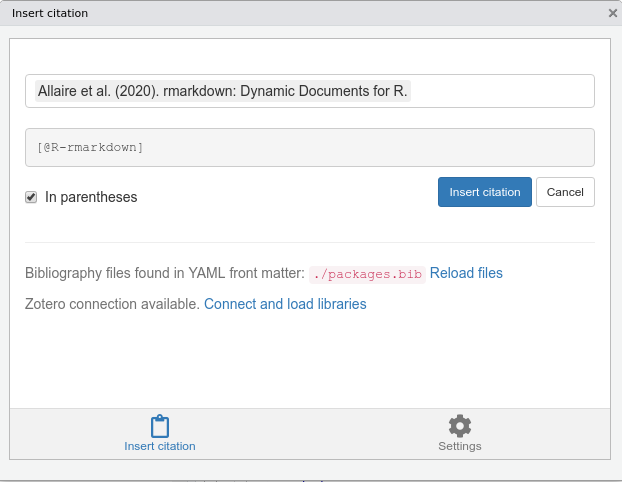
\includegraphics[width=0.5\linewidth]{img/citr} 

}

\caption{citrパッケージのGUI}\label{fig:citr-image}
\end{figure}

\end{frame}

\begin{frame}[fragile]{文献引用の補助: 文献管理}
\protect\hypertarget{ux6587ux732eux5f15ux7528ux306eux88dcux52a9-ux6587ux732eux7ba1ux7406}{}

\begin{itemize}
\tightlist
\item
  Mendeley, Zotero, ReabCubeの3つが多い?
\item
  私はZoteroを使っている

  \begin{itemize}
  \tightlist
  \item
    多言語対応, 連携機能の充実, 料金などの理由
  \item
    参考:
    『\href{https://ill-identified.hatenablog.com/entry/2019/03/05/195257}{Mendeley
    Exodus Mendeley から Zotero への移行の手引き\textasciitilde{}}』
  \end{itemize}
\item
  \texttt{RefManageR} パッケージ

  \begin{itemize}
  \tightlist
  \item
    Rでbibファイルをパースしたりする
  \item
    文献管理用には既存ソフトで十分?
  \end{itemize}
\end{itemize}

\end{frame}

\hypertarget{ux305dux306eux4ed6ux306eux6a5fux80fd}{%
\section{その他の機能}\label{ux305dux306eux4ed6ux306eux6a5fux80fd}}

\begin{frame}[fragile]{絵文字}
\protect\hypertarget{ux7d75ux6587ux5b57}{}

\begin{itemize}
\tightlist
\item
  \href{https://github.com/zr-tex8r/BXcoloremoji}{\texttt{BXcoloremoji}}をインストールすれば可能

  \begin{itemize}
  \tightlist
  \item
    \texttt{\textbackslash{}coloremoji\{\}} で絵文字表示:
    \ifdefined\coloremoji \coloremoji{🍣} \else (ここに絵文字) \fi
  \item
    RStudioエディタでは\textbf{表示が変な場合も}
  \end{itemize}
\item
  グラフ描画には特に設定必要なし

  \begin{itemize}
  \tightlist
  \item
    ソースコード上のものは文字化けする
  \end{itemize}
\end{itemize}

\begin{Shaded}
\begin{Highlighting}[]
\KeywordTok{plot}\NormalTok{(}\DecValTok{1}\OperatorTok{:}\DecValTok{10}\NormalTok{, }\DataTypeTok{pch =} \StringTok{"🍣"}\NormalTok{)}
\end{Highlighting}
\end{Shaded}

\begin{center}\includegraphics[width=0.5\linewidth]{presen_test_files/figure-beamer/sushi-plot-1} \end{center}

\end{frame}

\hypertarget{ux30c8ux30e9ux30d6ux30ebux30b7ux30e5ux30fcux30c6ux30a3ux30f3ux30b0}{%
\section{トラブルシューティング}\label{ux30c8ux30e9ux30d6ux30ebux30b7ux30e5ux30fcux30c6ux30a3ux30f3ux30b0}}

\begin{frame}[fragile]{エラーの原因がよくわからない}
\protect\hypertarget{ux30a8ux30e9ux30fcux306eux539fux56e0ux304cux3088ux304fux308fux304bux3089ux306aux3044}{}

\begin{itemize}
\tightlist
\item
  \textbf{キャッシュ削除すると良くなることもある}

  \begin{itemize}
  \tightlist
  \item
    (叩けば直るレベルのアドバイス)
  \item
    前回エラーで失敗したときのキャッシュが悪さしてることは結構ある
  \item
    または \texttt{cache\ =\ F} でキャッシュを残さないようにする
  \item
    エラーメッセージが実態と矛盾してるときはまず試す
  \end{itemize}
\end{itemize}

\end{frame}

\hypertarget{ux307eux3068ux3081}{%
\section{まとめ}\label{ux307eux3068ux3081}}

\begin{frame}[fragile]{結果どうなったか}
\protect\hypertarget{ux7d50ux679cux3069ux3046ux306aux3063ux305fux304b}{}

\begin{itemize}
\tightlist
\item
  \textbf{良く}なったこと

  \begin{itemize}
  \tightlist
  \item
    \texttt{lstlisting.sty}\textbf{より見やすい}シンタックスハイライト
  \item
    Rの画像や数値出力を\textbf{コピペしなくて済む}
  \item
    一画面に収めるための構成だけ考えれば済むように
  \end{itemize}
\item
  \textbf{悪く}なったこと

  \begin{itemize}
  \tightlist
  \item
    (パワポユーザ的に)WYSIWYGでないので作りづらい?
  \item
    数式のリアルタイムレンダリング/補完はLyXが依然優秀
  \item
    python作業中(jupyter notebookへの)\textbf{不満高まり}
  \item
    ポンチ絵も\texttt{ggplot2}で作らねばという\textbf{強迫症状}
  \end{itemize}
\end{itemize}

\end{frame}

\begin{frame}{改良したいところ}
\protect\hypertarget{ux6539ux826fux3057ux305fux3044ux3068ux3053ux308d}{}

\begin{itemize}
\tightlist
\item
  手動セットアップ作業の削減

  \begin{itemize}
  \tightlist
  \item
    例:
    \href{https://atusy.github.io/tokyor85-original-rmd-format}{ヘッダのテンプレート化}
  \end{itemize}
\item
  細かいレイアウト修正
\item
  他の言語のシンタックスハイライト
\item
  最低限のテーマ変更オプションの追加
\end{itemize}

\end{frame}

\hypertarget{ux7d30ux304bux3044ux6280ux8853ux7684ux306aux8a71}{%
\section{細かい技術的な話}\label{ux7d30ux304bux3044ux6280ux8853ux7684ux306aux8a71}}

\begin{frame}[fragile]{yamlヘッダ設定: 出力の設定}
\protect\hypertarget{yamlux30d8ux30c3ux30c0ux8a2dux5b9a-ux51faux529bux306eux8a2dux5b9a}{}

\begin{itemize}
\tightlist
\item
  \XeLaTeX 生成

  \begin{itemize}
  \tightlist
  \item
    \LuaLaTeX 使用者が多数派?
  \end{itemize}
\item
  ``\texttt{keep\_tex:\ true}'' エラー発生時の原因特定に
\end{itemize}

\begin{Shaded}
\begin{Highlighting}[]
\FunctionTok{output}\KeywordTok{:}
\AttributeTok{  }\FunctionTok{beamer_presentation}\KeywordTok{:}
\AttributeTok{    }\FunctionTok{latex_engine}\KeywordTok{:}\AttributeTok{ xelatex}
\AttributeTok{    }\FunctionTok{citation_package}\KeywordTok{:}\AttributeTok{ natbib}
\AttributeTok{    }\FunctionTok{keep_tex}\KeywordTok{:}\AttributeTok{ }\CharTok{true}
\end{Highlighting}
\end{Shaded}

\end{frame}

\begin{frame}[fragile]{\LaTeX プリアンブル: テーマ設定}
\protect\hypertarget{ux30d7ux30eaux30a2ux30f3ux30d6ux30eb-ux30c6ux30fcux30deux8a2dux5b9a}{}

\begin{itemize}
\tightlist
\item
  metropolisテーマを使用

  \begin{itemize}
  \tightlist
  \item
    \url{https://github.com/matze/mtheme}
  \item
    他のモダンなテーマは\emph{日本語と相性悪い}
  \item
    ``\texttt{beamer\_presentation:}''
    内で指定すると\textbf{オプション指定できない}
  \end{itemize}
\end{itemize}

\begin{Shaded}
\begin{Highlighting}[]
\FunctionTok{header-includes}\KeywordTok{:}
\AttributeTok{  }\KeywordTok{-}\AttributeTok{ \textbackslash{}usetheme[progressbar=frametitle,block=fill]\{metropolis\}}
\AttributeTok{  }\KeywordTok{-}\AttributeTok{ \textbackslash{}makeatletter}
\AttributeTok{  }\KeywordTok{-}\AttributeTok{ \textbackslash{}setlength\{\textbackslash{}metropolis@progressinheadfoot@linewidth\}\{2pt\}}
\AttributeTok{  }\KeywordTok{-}\AttributeTok{ \textbackslash{}usefonttheme\{professionalfonts\}}
\end{Highlighting}
\end{Shaded}

\end{frame}

\begin{frame}[fragile]{\LaTeX プリアンブル: 日本語フォント設定}
\protect\hypertarget{ux30d7ux30eaux30a2ux30f3ux30d6ux30eb-ux65e5ux672cux8a9eux30d5ux30a9ux30f3ux30c8ux8a2dux5b9a}{}

\begin{itemize}
\tightlist
\item
  \texttt{zxjatype} で日本語フォント読み込み

  \begin{itemize}
  \tightlist
  \item
    \texttt{mainfont:\ \textless{}HOGEHOGE\textgreater{}} も可
  \item
    しかし欧文和文で別にしたい
  \end{itemize}
\item
  和文欧文サイズ比調整などは\href{http://zrbabbler.sp.land.to/zxjatype.html}{開発者のサイト}等参照
\end{itemize}

\begin{Shaded}
\begin{Highlighting}[]
\KeywordTok{-}\AttributeTok{ \textbackslash{}usefonttheme\{professionalfonts\}}
\KeywordTok{-}\AttributeTok{ \textbackslash{}usepackage\{zxjatype\}}
\KeywordTok{-}\AttributeTok{ \textbackslash{}setmainfont[Ligatures=TeX]\{Palatino Linotype\}}
\KeywordTok{-}\AttributeTok{ \textbackslash{}setsansfont[Ligatures=TeX]\{Arial\}}
\KeywordTok{-}\AttributeTok{ \textbackslash{}setmonofont\{Ricty Diminished\}}
\KeywordTok{-}\AttributeTok{ \textbackslash{}setjamainfont\{Noto Serif CJK JP\}}
\KeywordTok{-}\AttributeTok{ \textbackslash{}setjasansfont\{Noto Sans CJK JP\}}
\KeywordTok{-}\AttributeTok{ \textbackslash{}setjamonofont\{Ricty Diminished\}}
\end{Highlighting}
\end{Shaded}

\end{frame}

\begin{frame}{\LaTeX プリアンブル: その他の設定}
\protect\hypertarget{ux30d7ux30eaux30a2ux30f3ux30d6ux30eb-ux305dux306eux4ed6ux306eux8a2dux5b9a}{}

\begin{itemize}
\tightlist
\item
  ハイパーリンクの色を見やすく変更
\item
  ``Figure 1'', ``Table 1'' を 「図1」「表1」に
\item
  参考文献リストのフォントサイズ縮小
\item
  コードチャンクに行番号

  \begin{itemize}
  \tightlist
  \item
    表示は選択式
  \end{itemize}
\item
  その他いろいろな微調整
\end{itemize}

\end{frame}

\begin{frame}[fragile]{日本語文献にどう対応しているか}
\protect\hypertarget{ux65e5ux672cux8a9eux6587ux732eux306bux3069ux3046ux5bfeux5fdcux3057ux3066ux3044ux308bux304b}{}

\begin{itemize}
\tightlist
\item
  \href{https://github.com/ShiroTakeda/jecon-bst/blob/master/jecon.bst}{\texttt{jecon.bst}}を使いたい

  \begin{itemize}
  \tightlist
  \item
    \BibTeX はマルチバイト文字未対応
  \item
    \upBibTeX が必要
  \end{itemize}
\item
  \texttt{knitr}は日本語書誌情報処理未対応

  \begin{itemize}
  \tightlist
  \item
    内部では自前の設定で\texttt{latexmk}を呼び出し
  \item
    呼び出しているラッパにオプションがない
  \item
    積極的に改修の気配なし(\href{https://github.com/yihui/tinytex/issues/70}{参考})
  \end{itemize}
\item
  自前の設定を使用する(\href{https://github.com/kenjimyzk/bookdown_ja_template}{参考})

  \begin{itemize}
  \tightlist
  \item
    \texttt{tinytex.latexmk.emulation\ =\ F}
  \item
    \href{https://texwiki.texjp.org/?Latexmk}{ここ}を参考に\texttt{.latexmkrc}設定
  \item
    \textbf{Rmdと同じディレクトリに}上記を置く
  \end{itemize}
\item
  もっとシンプルな方法を\textbf{検討中}
\end{itemize}

\end{frame}

\begin{frame}[fragile]{些細だが気に入らないこと(試行錯誤中)}
\protect\hypertarget{ux4e9bux7d30ux3060ux304cux6c17ux306bux5165ux3089ux306aux3044ux3053ux3068ux8a66ux884cux932fux8aa4ux4e2d}{}

\begin{itemize}
\tightlist
\item
  番号式の引用子の設定方法

  \begin{itemize}
  \tightlist
  \item
    \texttt{citation\_package="natbib"}指定した上で\texttt{\textbackslash{}usepackage{[}number{]}\{natbib\}}
  \item
    前者を指定しないと\BibTeX を使わない仕様?
  \end{itemize}
\item
  逆にテーマのオプションは\texttt{render(theme=)}に指定不可

  \begin{itemize}
  \tightlist
  \item
    二重定義はエラーの原因になるため
  \end{itemize}
\item
  自作beamerテンプレと比較して微妙にフォントサイズが違う(なぜ?)
\item
  相互参照機能

  \begin{itemize}
  \tightlist
  \item
    \href{https://stackoverflow.com/questions/54041552/impossible-to-cross-referring-figures-and-tables-with-beamer-presentation-opti}{こういう方法}でできるらしい
  \end{itemize}
\item
  面倒な下準備せずに\upBibTeX 使いたい
\end{itemize}

\end{frame}

\renewcommand\refname{参考文献}
\begin{frame}[allowframebreaks]{参考文献}
  \bibliographytrue
  \bibliography{references.bib}
\end{frame}

\end{document}
